\subsection{Kinematics}
We begin our study of mechanics by trying to quantify the behavior of moving objects. Specifically, we will look at how objects' position, velocity, and acceleration are related, and how these can be used to solve problems involving motion, especially in certain special cases. 
\subsubsection{General Motion}
Moving forward, we will describe an object's position using a vector with respect to some point, denoted $\vec{r}$. For simplicity, we will use a point as our moving particle, but principles here really apply to any object. \\
\begin{center}
	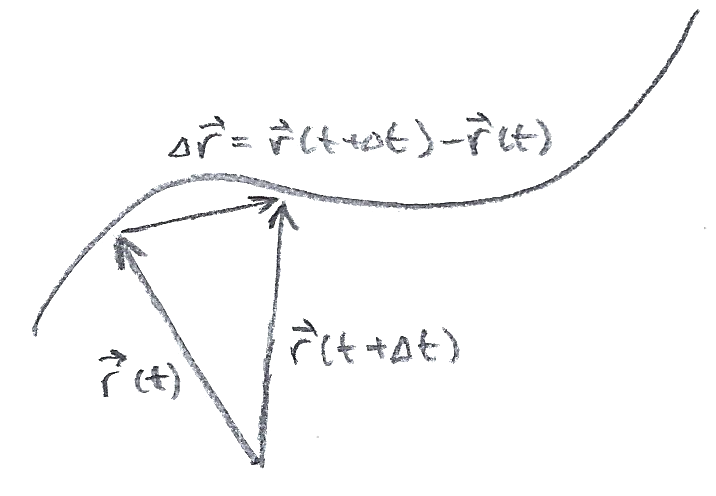
\includegraphics[width=0.5\textwidth]{images/mechintro/general_motion.png}\\
\end{center}
Knowing the position of the object is great, but we would definitely like to know more about a particle than just its position. For example, how do we know how fast is the particle going? Intuitively, we can find the average velocity of a particle over an interval by taking the distance traveled over the time interval. Consider the particle at two different times, with positions $\vec{r}(t)$ and $\vec{r}(t + \Delta t)$. Define the displacement of the particle as $\Delta\vec{r} = \vec{r}(t + \Delta t) - \vec{r}(t)$. Using the displacement vector, we can find the average velocity (a vector): 
\[
	\vec{v}_{av} = \frac{\Delta \vec{r}}{\Delta t} = \frac{\vec{r}(t + \Delta t) - \vec{r}(t)}{\Delta t}
\]
Average velocity is nice, but we would like to know the velocity instantaneously. Notice as we shrink the time interval $\Delta t$, our average velocity becomes more and more like the instantaneous velocity $\vec{v}$. In the limit as $\Delta t \rightarrow 0$, we have:
\[
	\vec{v} = \lim_{\Delta t \rightarrow 0} \frac{\vec{r}(t + \Delta t) - \vec{r}(t)}{\Delta t}
\]
This looks rather like the derivative of the position vector function $\vec{r}(t)$ with respect to time! However, we don't really know how to take the derivative of a vector, but we \textit{should} know how to take the derivative of an arbitrary function. We can actually do this by splitting the position vector $\vec{r}(t)$ into $xy$-components, where $\vec{r}(t) = x(t) \hat{x} + y(t) \hat{y}$ and $\vec{r}(t+\Delta t) = x(t+\Delta t) \hat{x} + y(t+\Delta t) \hat{y}$:
\begin{align*}
	\vec{v}(t) &= \lim_{\Delta t \rightarrow 0} \frac{x(t+\Delta t) \hat{x} + y(t+\Delta t) \hat{y} -x(t) \hat{x} -y(t) \hat{y}}{\Delta t}\\
	&= \lim_{\Delta t \rightarrow 0} \frac{x(t+\Delta t)-x(t)}{\Delta t} \hat{x} + \lim_{\Delta t \rightarrow 0}\frac{y(t+\Delta t)-y(t)}{\Delta t} \hat{y}\\
	&= \dv{x}{t}\hat{x} + \dv{y}{t} \hat{y} = v_x\hat x + v_y \hat y
\end{align*}
Note that $v_x = \dv{x}{t}$ is the $x$-component of the velocity, and $v_y = \dv{y}{t}$ is the $y$-component of the velocity. We can do this process again to attain the instantaneous acceleration vector $\vec a$, noting that the average acceleration is the change in the velocity vector over a time $\Delta t$ and allowing $\Delta t$ to go to $0$:
\[
	\vec a = \dv{v_x}{t}\hat x + \dv{v_y}{t} \hat y = \ddv{x}{t} \hat x + \ddv{y}{t} \hat y
\]
We normally don't deal with any derivatives of position (with respect to time) of order higher than two. Also, usually we will deal with constant-acceleration motion and constant-velocity (zero acceleration) motion, with some special exceptions. More general cases will be dealt with later when we discuss energy. \\
Let's deal with the constant-velocity case right now. Because of the Fundamental Theorem of Calculus, we can note the following: 
\[
	x(t) - x_0 = \int_0^t v_x \, dt = v_xt \rightarrow x(t) = v_xt + x_0
\]
where the last step follows from noting that the velocity is a constant, and therefore so are each component of the velocity vector. Using similar relations for the $y$-coordinate, we have: 
\[
	\vec r(t) = \vec v t + \vec r_0
\]
We don't need any other information about constant-velocity problems - since the velocity is constant, all higher order derivatives must be zero.\\
Now we look at the constant-acceleration case, starting with the acceleration vector $\vec a$. We can use the Fundamental Theorem of Calculus again, as we did with the constant-velocity case: 
\[
	v_x(t) - v_{0_{x}} = \int_0^t a_x \, dt = a_xt \rightarrow v_x(t) = a_xt + v_{0_{x}}
\]
Repeating this again, we can find the $x$-coordinate of position:
\[
	x(t) - x_0 = \int_0^t v_x \, dt = \int_0^t v_{0_{x}} + a_xt \, dt = v_{x0}t + \frac{1}{2}at^2  \rightarrow x(t) = x_0 + v_{0_{x}}t + \frac{1}{2}at^2
\]
Using similar processes for the $y$-coordinate, we have
\[
	\vec{r}(t) = \vec r_0 + \vec v_0 t + \frac{1}{2} \vec{a} t^2 
\]
\[
	\vec v(t) = \vec a t + \vec v_0
\]
where $\vec r_0$ is the initial position vector, $\vec v_0$ is the initial velocity vector, and $\vec a$ is the acceleration vector. \\
These equations work fine unless we don't have access to time data. However, we can derive a constant-acceleration equation that does not involve time, using one dimension for simplicity. We can square our general equation for velocity: 
\begin{align*}
	v &= at + v_0 \\
	v^2 &= a^2t^2 + v_0^2 + 2atv_0 \\
	v^2 - v_0^2 &= 2a\left(\frac{1}{2}at^2 + v_0t \right)
\end{align*}
This expression in the parentheses is familiar - note the displacement can be written as:
\[
	\Delta x = x(t) - x_0 = \frac{1}{2}at^2 + v_0t
\]
Now we have a kinematic equation that does not deal with time: 
\[
	v^2 - v_0^2 = 2a\Delta x
\]
Note that these equations are the same in higher dimensions (for example, in 3D space) and are derivable with the same procedures and steps. 

\subsubsection{Circular Motion}
A special type of motion that we will study is circular motion. In order to derive the equations for this motion, we use polar coordinates. We can parameterize the points in the plane with the angle it makes with the positive $x$-axis and the distance from the origin. Let $\theta(t)$ be this angle as a function of time, and we can express the position of a point in the plane as $\vec r = r \cos (\theta (t)) \, \hat x + r \sin (\theta (t)) \, \hat y$, where $r$ is the constant radius of the circle the particle travels upon. In addition to $\hat x$ and $\hat y$, constant unit vectors, we define changing unit vectors $\hat r$ and $\hat \theta$, where $\hat r$ is radially outward and $\hat \theta$ is the unit vector perpendicular to it, defined as follows: \\
\[
	\hat r = \cos (\theta (t)) \, \hat x + \sin (\theta (t)) \, \hat y 
\]
\[
	\hat \theta = -\sin (\theta (t)) \, \hat x + \cos (\theta (t)) \, \hat y
\]
\begin{center}
	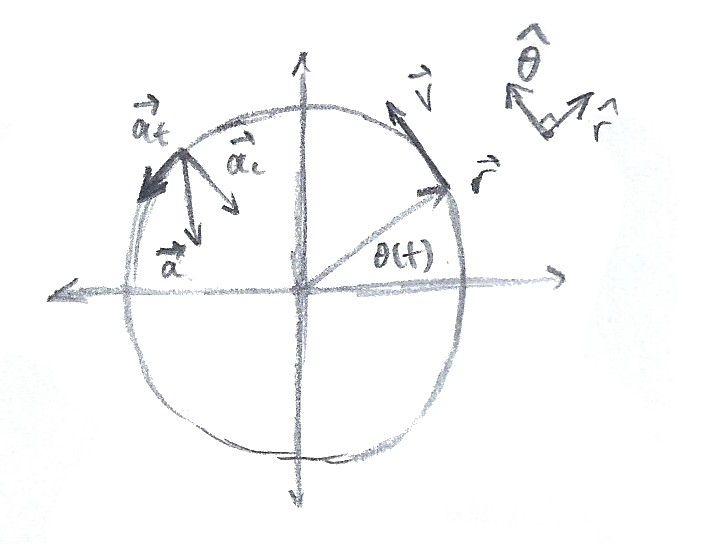
\includegraphics[width=0.5\textwidth]{images/mechintro/circular_motion.png}\\
\end{center}
We can take the derivative of the position vector in order to find the velocity of the object, using the method in the previous section: 
\[
	\vec v = \dv{\vec r}{t} = - r \sin (\theta (t)) \, \dv{\theta}{t} \, \hat x + r \cos (\theta (t)) \, \dv{\theta}{t} \, \hat y
\]
Notice by the chain rule an extra $\omega = \dv{\theta}{t}$ appears in each term; this term is called the angular velocity. We can rewrite $\vec v$ as follows: 
\[
	\vec v = \omega r (-\sin (\theta (t)) \, \hat x + \cos (\theta (t)) \, \hat y) 
\]
The acceleration of the object is a bit messy, but we can take derivatives again, substituting $\alpha = \dv{\omega}{t}$: 
\begin{align*}
	\vec a = \dv{\vec v}{t} &= -r \left(\dv{\omega}{t}\sin (\theta (t)) + \omega^2 \cos (\theta (t)) \right) \hat x + r \left(\dv{\omega}{t} \cos (\theta (t)) - \omega^2 \sin (\theta (t)) \right) \hat y \\
	&= \alpha r (-\sin (\theta (t)) \, \hat x + \cos (\theta (t)) \, \hat y) - \omega^2 r (\cos (\theta (t)) \, \hat x + \sin (\theta (t)) \, \hat y) 
\end{align*}
This is all pretty messy, but we can clean up these expressions by using $\hat r$ and $\hat \theta$: 
\begin{align*}
	\vec r &= r \hat r \\
	\vec v &= \omega r \hat \theta \\
	\vec a &= \alpha r \hat \theta - \omega^2 r \hat r
\end{align*}
Observe that since these unit vectors have magnitude $1$, so the velocity $v = \omega r$, with direction tangent to the circle. We should notice for cases with non-constant acceleration, we have a centripetal component ($-\omega^2 r \hat r$, pointing radially inward) and a tangential component ($\alpha r \hat \theta$, tangent to the circle).
A special case we study is when $\omega$ is a constant, implying that $\alpha = 0$. This is called uniform circular motion, and we see for this case the only acceleration is centripetal: 
\[
	\vec a = - \omega^2 r \hat r = - \frac{v^2}{r} \hat r 
\]
Overall, we have, for uniform circular motion (for the magnitudes of the velocity and angular velocity):
\begin{align*}
	v &= \omega r \\
	a &= \omega^2 r = \frac{v^2}{r}
\end{align*}

\subsubsection{Simple Harmonic Motion (SHM)}
Consider projecting circular motion into one dimension - namely, only considering the $x$-direction. This one-dimensional motion can basically be modeled by the function $x(t) = A \cos(\omega t + \phi)$, where $A$ is the amplitude, $\omega$ is the frequency/angular velocity, and $\phi$ is the phase shift. This is simple harmonic motion, which essentially uses a sine/cosine function as a model for motion. \\
Using our knowledge of derivatives, the velocity and acceleration functions: 
\begin{align*}
	v(t) &= -\omega A \sin(\omega t + \phi) \\
	a(t) &= -\omega^2 A \cos(\omega t + \phi) 
\end{align*}
We'll do something somewhat unorthodox - we'll substitute $x(t)$ for the cosine function in the acceleration function, giving: 
\[
	a(t) = \ddv{x}{t} = -\omega^2 x(t)
\]
In general, if given an acceleration function proportional to position, where $a(t) = -kx(t)$, we know the particle exhibits simple harmonic motion (sine/cosine wave) where $\omega = \sqrt{k}$ and the period $T = \frac{2\pi}{\omega} = \frac{2\pi}{\sqrt{k}}$. \\
Mathematically, if a second derivative of a function $\ddv{f}{t} = -kf$, the function $f$ can be modeled as a sine or cosine function. 

\subsubsection{Projectile Motion and Relative Motion}
We can apply general 2-D motion principles to projectiles. Let a particle be launched at an angle $\theta$ at an initial velocity $v_0$. Note that this particle is constantly accelerating downward with magnitude $g = 9.81 \, m/s^2$. To make things simpler, we will automatically project into the $x$- and $y$- directions, with the implication that we are in fact dealing with vectors. Also, further assumptions that we make is that the Earth's gravitational acceleration is uniform at all heights - which clearly isn't true in outer space - but otherwise we have non-constant acceleration which we haven't learned to deal with yet. We also neglect air resistance, which changes the acceleration of the particle. \\
The initial velocity in the $x$-direction is $v_0 \cos \theta$, and the initial velocity in the $y$-direction is $v_0 \sin \theta$. Plugging into our derived time-dependent kinematic equations, and letting the initial position be the origin: 
\[
	x(t) = v_0t\cos\theta  \quad v_x(t) = v_0\cos\theta
\]
\[
	y(t) = v_0t\sin\theta  - \frac{1}{2}gt^2 \quad v_y(t) = v_0 \sin \theta - gt
\]
We can analyze some critical points - we can calculate how far the particle will travel before it hits the ground, namely when $y = 0$. When this is the case, we have: 
\[
	v_0t\sin\theta  - \frac{1}{2}gt^2 = 0 \rightarrow v_0\sin\theta - \frac{1}{2}gt = 0
\]
This equation has a zero when $t=0$, and solving the remaining linear equation yields $t = \frac{2v_0\sin\theta}{g}$. When this is plugged into $x(t)$, we have $\frac{2v_0^2\sin\theta \cos\theta}{g} = \frac{v_0^2\sin 2\theta}{g}$.\\
Similarly, we can consider when the particle reaches its maximal height. Clearly, by symmetry we have that the distance that the particle had traveled to that point is $\frac{v_0^2\sin \theta \cos\theta}{g}$. However, we can find the maximal height by calculating the time when the $y$-component of the velocity is $0$, where the particle stops going upward and begins to fall back to earth. This occurs when:
\[
	v_0\sin\theta - gt = 0 \rightarrow t = \frac{v_0\sin\theta}{g}
\]
Note that the time when this occurs is exactly half of the time it takes for the particle to hit the ground. When this occurs, the height can be calculated by plugging into $y(t)$, where $y(t) =\frac{v_0^2\sin^2\theta}{2g}$. \\
Of course, this is all well and good, but we do need to be able to consider when things hit each other, especially with projectiles (which is a very common problem). \\
\begin{center}
	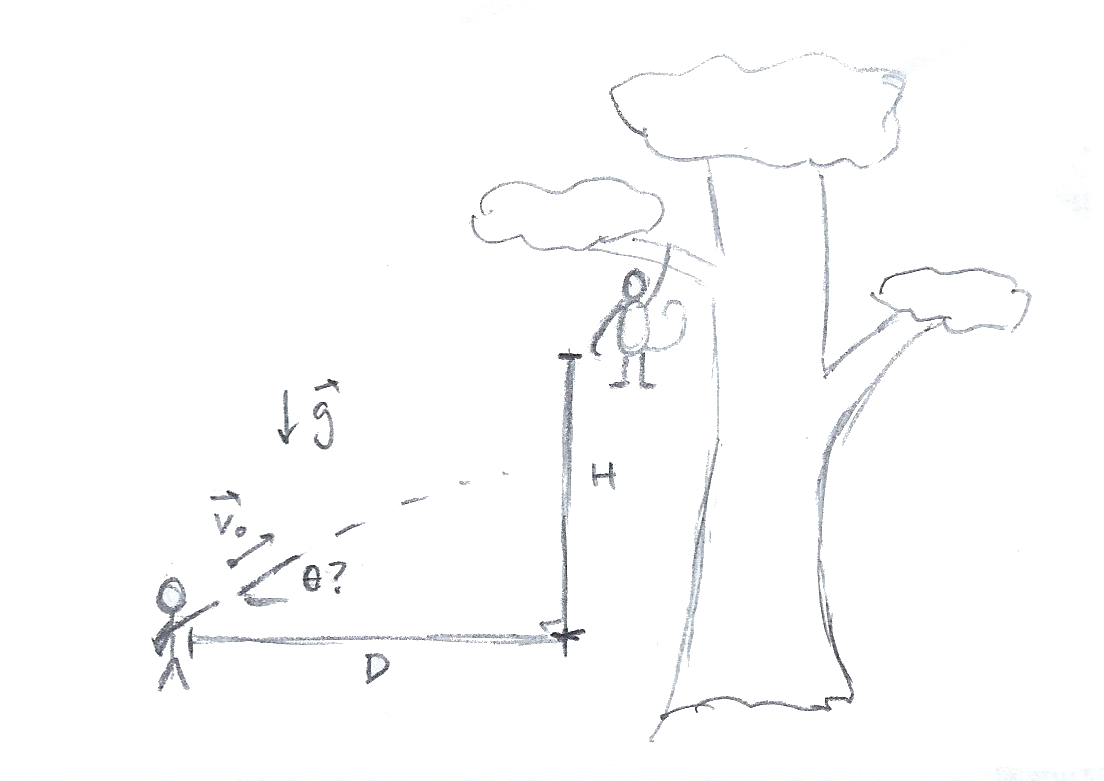
\includegraphics[width=0.5\textwidth]{images/mechintro/projectile_motion.png}\\
\end{center}
We can use kinematics to solve problems - one of the first applications was used for hunting, because animal cruelty organizations didn't exist when physics was invented. For example, suppose a hunter stands a distance $D$ away from the base of a tree, in which a monkey is sitting at the top, hanging from a branch. The monkey is hanging at a height $H$, and the hunter can shoot a bullet at the monkey with velocity $v_0$. We're trying to find at what angle $\theta$ should the hunter fire to hit the monkey. We're also assuming the monkey is effectively a point, and at the instant the hunter fires, the monkey lets go of the branch and begins to fall freely with downward acceleration with magnitude $g$.\\
Consider the position vector of the monkey relative to the bullet, $\vec r_{MB}$. To deal with this, we employ the following, where $O$ is some arbitrary origin we've been using the entire time:
\[
	\vec r_{BO} + \vec r_{MB} = \vec r_{MO} \rightarrow \vec r_{MB} = \vec r_{MO} - \vec r_{BO} 
\]
To compute the relative position vector, then, we really only need to 
compute the position vectors of the monkey and the bullet and subtract them. We know they collide when their relative position vector is the zero vector $\vec 0$.  We know how both of these particles work - effectively, they are both projectiles, which we have just established. For simplicity, let the position of the hunter be the origin. Then, we have: 
\[
	\vec r_{MO} = D\, \hat x + \left(H - \frac{1}{2}gt^2 \right)\, \hat y \quad \vec r_{BO} = v_0t\cos\theta \, \hat x + \left(v_0t\sin\theta - \frac{1}{2} gt^2 \right) \, \hat y
\]
Then their relative position is: 
\[
	\vec r_{MB} = (D - v_0t\cos\theta) \, \hat x + (H - v_0t\sin\theta) \, \hat y
\]
When this is the zero vector, we have that both components are zero, giving:
\[
	\cos \theta = \frac{D}{v_0t} \quad \sin \theta = \frac{H}{v_0t} \rightarrow \tan \theta = \frac{H}{D}
\]
This angle is the exact angle at which the hunter should shoot the monkey hanging from the tree, given our assumptions. Therefore, the hunter should aim directly at the monkey, as long as the bullet is traveling fast enough to reach the tree before the monkey hits the ground. 

\subsubsection{Summary and Problems}
Position, velocity, and acceleration of objects can be represented by a vector with respect to a point. Velocity is the derivative with respect to time of position, and acceleration is the derivative with respect to time of velocity (and the second derivative with respect to time of position). Position and velocity can be attained through velocity or acceleration functions, respectively, through integration. \\
We deal with a few special cases, being (uniform) circular motion, simple harmonic motion, and projectile motion. These are situations that we should be proficient in before moving forward to more complex motion and systems. \\

\noindent \textbf{Problems:}\\
1. (3 $\bigstar$) At $1/2$ of its maximum height, the speed of a projectile is $3/4$ of its initial speed. If the particle was initially launched at an angle $\theta$, where $\theta = \arctan(x)$, show that $x = \sqrt{7}$.\\
2. (2 $\bigstar$) A boy whirls a stone in a horizontal circle of radius $r$ and at height $h$ above ground level. The string breaks, and the stone flies horizontally and strikes the ground after traveling a horizontal distance of $d$. Show the magnitude of the centripetal acceleration of the stone while in circular motion is $d^2g/2hr$. \\
3. (2 $\bigstar$) Two particles oscillate in simple harmonic motion along a common straight-line segment of length $A$. Each particle has a period of 3.80 s, but they differ in phase by $\pi/8$ rad. a) Show the maximum acceleration and velocities of the particles are 2.734$A$ and 1.653$A$, respectively. b) Show the particles are 0.167$A$ apart $0.50$ s after the lagging particle leaves one end of the segment.\\
4. (1 $\bigstar$) A tank fires a rocket at a velocity $v_r$ at an angle $\theta$ above the horizontal. Immediately afterward, the tank begins moving forward at a constant speed $v_t$. Show that the angle of stupidity $\theta$ of the tank - that is, the angle at which the rocket will fall down to strike the tank while on the ground - as $\arccos(v_t/v_r)$. \\
5. (3 $\bigstar$, $\spadesuit$) A small rock sinking through water experiences an exponentially decreasing acceleration given by $a_y(t) = ge^{-bt}$, where $b$ is a positive constant that depends on the shape/size of the rock and the properties of the water. If the initial position and velocity of the rock are both zero, find the a) velocity function to be $v_y(t) = \frac{g}{b} (1-e^{-bt})$. b) the position function to be $y(t) = \frac{g}{b}t - \frac{g}{b^2}(1-e^{-bt})$.\\
6. (2 $\bigstar$) Prove that if two particles are launched at the same speed $v_0$ but at angles above the horizontal that exceed/fall short of 45 degrees by the same amount, they will still travel the same distance (on level ground).\\
7. (3 $\bigstar$) If two balls are thrown with the same initial speed $v_0$ but at different angles $\alpha$ and $\beta$ above and below the horizontal, respectively, and from a cliff a height $h$ above the ground, show that their velocities right before they hit the ground are the same and is equal to $v = \sqrt{v_0^2+2gh}$.\\

\pagebreak